\documentclass[10pt]{standalone}
\usepackage{amsmath}
\usepackage{pgf,tikz}
\usepackage{mathrsfs}
\usetikzlibrary{arrows}
\pagestyle{empty}
\begin{document}


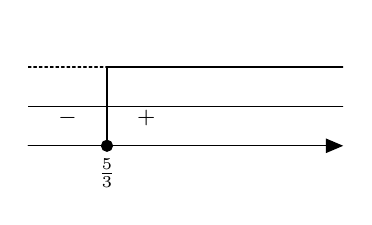
\begin{tikzpicture}[line cap=round,line join=round,>=triangle 45,x=1.0cm,y=1.0cm]
\draw[->] (-2.,0.) -- (2.,0.);


% 2/02/2018 :: 9:42:21 :: \draw (0pt,-10pt) node {\footnotesize $0$};
\draw (-1,-10pt) node {\footnotesize $\frac{5}{3}$};
\draw (-1.5,10pt) node {\footnotesize $-$};
% 2/02/2018 :: 9:41:20 :: \draw (0.5,10pt) node {\footnotesize $+$};
\draw (-0.5,10pt) node {\footnotesize $+$};
\clip(-2.,-0.5) rectangle (2.,1.5);
\draw  (-1.,0.)-- (-1.,1.);
\draw [dash pattern=on 1pt off 1pt] (-2.,1.)-- (-1.,1.);
\draw  (-1.,1.)-- (2.,1.);
\draw  (0.,0.5)-- (-2.,0.5);
\draw  (0.,0.5)-- (2.,0.5);
% 2/02/2018 :: 9:44:55 :: \draw  (0.,0.5)-- (0.,0.);
% 2/02/2018 :: 9:40:32 :: \draw  (-2.,1.5)-- (2.,1.5);
\begin{scriptsize}
\draw [fill=black] (-1.,0.) circle (2.0pt);
% 2/02/2018 :: 9:43:35 :: \draw  (-1.,1.) circle (2.0pt);
% 2/02/2018 :: 9:42:34 :: \draw  (0.,0.5) circle (2.0pt);
% 2/02/2018 :: 9:42:54 :: \draw [fill=black] (0.,0.) circle (2.0pt);
\end{scriptsize}
\end{tikzpicture}
\end{document}